\chapter{Variables In C}
When we want to store data to memory in assembly, we write to raw memory addresses. 
"Store this value to this address."
This obviously minimises the portability of our code as we would have to modify all of the memory addresses if we ported our code to a different system with a different memory architecture.
Instead of having to interface with memory directly, a more abstract language like C allows us to define and use \emph{variables}. 

A variable essentially allows you to give some memory a name and specify what operations can be done on that block of memory.
The amount of memory which the variable will be allocated and the operations which can be done to it are specified by the variable's \emph{data type}. 

One of the main advantages of using variables is that you do not need to specify or keep track of where your data will be stored in memory. The compiler\footnote{Technically it's the \emph{linker} which actually maps variable names to absolute memory addresses. Prior to linking, the memory addresses are all relative to segments.} keeps track of the mapping between the variable name and the memory addresses associated with that variable name.

\section{Types}
As mentioned earlier, the variable type specifies the amount of memory space which must be allocated for the variable and what operations can be done with or on that memory. The general format of a variable declaration is as follows.

\begin{lstlisting}[language=C]
type name = value;
\end{lstlisting}

We will now proceed to explore two of the most common types.

\subsection{Basic Types}
Basic types specify a block of memory which is treated as a simple number. While you do get basic types which support decimals, for most of our applications, the number will only be an integer. Much like how we had word, half-word or byte data types in assembly, we have similar number types in C.

C programmers frequently specify their types as either \texttt{char}, \texttt{int}, \texttt{short} or \texttt{long}. The problem with this is that the actual size of each of these types is not consistant across platforms. 
For example, the size of an \texttt{int} on your computer will be either 32 bits and 64 bits depending on which operating system you're running.

This ambiguity is an issue for us when working with microcontrollers. We often need to know exactly how much memory will be allocated to a variable. In order to specify the size of an int type exactly, we use the type definition \texttt{intx\_t} where \texttt{x} is either 8, 16, 32 or 64 and specifies the number of bits which must be allocated to that variable. The \texttt{\_t} indicates that it's a custom type which is defined in the \texttt{stdint.h} library. 

For example, the following definition will allocate 2 bytes of memory and call it \texttt{foo}.

\begin{lstlisting}[language=C]
int16_t foo;
\end{lstlisting}

The data held in the variable can either be treated as signed or unsigned data.
If a \texttt{u} is appended to the type the data should be treated as unsigned.
If no \texttt{u} is present the data should be treated as signed.

For example, in the following case \texttt{bar} is a signed number while \texttt{foo} is an unsigned number. 
\begin{lstlisting}[language=C]
uint32_t foo;
int32_t bar;
\end{lstlisting}

\subsection{Pointer Types}
We often want to deal with the memory addresses of variables or access specific addresses (such as in the case of interfacing with peripherals). For this, we can use pointer types. A pointer holds the address of some data. In other words, it point to some data.
The amount of data which is pointed to by the pointer is specified by the type. This means we need to specify two things when defining pointer types: we need to specify that the variable is a pointer type and we need to specify how much data is being pointed to.
We specify that it is a pointer using the asterisk. It is good practice to put the asterisk next to the variable name rather than next to the type.
For example, a pointer to 1 byte of data would be defined as follows\footnote{We specify the type again in brackets to do an explicit type cast. This is just to prevent a compiler warning by telling the compiler that we are intentionally (rather than accidentally) assigning a number to a pointer. Without the typecast, we would be assigning a basic type to a pointer type which would generate a warning.}.

\begin{lstlisting}[language=C]
int8_t *foo = (int8_t *)0x08001234;
\end{lstlisting}

Here, we are saying that the memory allocated to \texttt{foo} should point to the byte of data located at address.
Our address space runs from 0x0000 0000 to 0xFFFF FFFF which means that we need 4 bytes to store an address. Hence, no matter what the size of the data being pointed to is, a pointer type variable will always occupy 4 bytes in memory\footnote{This is architecture dependant though. A system which had a smaller or larger address space would require a different amount of data to be allocated for pointers.}.

Once we have a variable of type pointer, we are able to access the data being pointed to by the pointer with the dereference operator which is also an asterisk! This means that the asterisk has two possible meanings depending on context. If it's used during a variable declaration, it means the variable is of pointer type. If it is used on an existing variable of pointer type is means that we are accessing the data pointed to by the pointer, rather than accessing the pointer itself.

The following example shows defining a pointer, getting it to point to the address 0x2000 0550 and then modifying the data which is being pointed to.
\begin{lstlisting}[language=C]
uint32_t *bar;
bar = (uint32_t *)0x20000500;
*bar = 0xAABBCCDD;
\end{lstlisting}

The way arithmetic operations apply to pointers is different to the way arithmetic operations apply to basic types. With pointers, when you add or subtract values from the pointer, it actually adds or subtracts the value multiplied by the size of the data being pointed to. This can be thought of as causing the pointer to point to the next element of that type in memory, rather than just the next address.

A trivial example is shown below.
\begin{lstlisting}[language=C]
uint32_t  foo = 0x11223344;
uint32_t *bar = 0x11223344;
foo = foo - 1;   // foo now holds 0x11223343
bar = bar - 1;   // bar now holds 0x11223340
\end{lstlisting}

\subsection{Referencing}
We know that the address of variables is defined by the compiler. Suppose we want to ask the compiler what address it has assigned to a variable, how can we do that? The answer is by \emph{referencing} the variable. We've encountered dereferencing which essentially says "give me the data pointed to by this pointer." Referencing is the opposite process; it says "give me a pointer which points to this data." 

The reference operator is the ampersand operator. The datatype of a referenced variable is a pointer to the original type of the variable.
For example, the following defines a 8-bit integer \texttt{foo}, and then a pointer to an 8-bit integer \texttt{bar} which is then made to point to \texttt{foo}.

\begin{lstlisting}[language=C]
uint8_t foo = 0xAA;
uint8_t *bar;
bar = &foo;         // bar takes on the address of foo.
\end{lstlisting}

\section{Memory Allocation}
We now know that we can declare variables of different types which results in different amounts of memory being allocated to that variable. 
The question is, where does that memory get allocated?
Obviously, it must happen somewhere in RAM, as RAM is the block of memory which we use for general purpose data storage. 

The place is RAM which is used for the variable is determined by the storage duration or lifetime of the variable. 
There are two storage duration classes for variables: static and automatic. These will now be explored. 

\section{Automatically Allocated Variables}
We frequently only need a variable for some a short duration, such as when some function is called so that the variable can be used for storing intermediate data needed in the algorithm of the function.
When the function completes (returns) then that variable is no longer needed.
For this use-case, \emph{automatic} variables exist. 
These are variables which are only have memory allocated for them when a function call happens and are automatically deallocated on return. 
Automatic variables are those which are defined inside a function without the \texttt{static} keyword. Any variable defined inside a function is called a local variable and is only visible within that function. This is as opposed to a global variable which is visible to all functions. 
The great advantage of automatic variables is that by only occupying memory for a short time we are able to make more efficient use of memory. 

Where do automatic variables get allocated in memory? Well, they need to be somewhere that easily supports the dynamic allocation and deallocation of memory. This is exactly that the stack does! When you \texttt{PUSH} a value to the stack it allocates some memory. When you \texttt{POP} a value it deallocates space on the stack. As such, the stack is used for automatic variables.

When a function call happens, the first things that the function does is allocates space for all of its automatic variables\footnote{More accurately, it's actually when a block is entered into, any variables defined in that block are allocated.}. How? The stack pointer is decremented by some amount to make space on the stack for all of the variables. The compiler keeps track of which spot on the stack maps to which variable name. If any of those automatica variables have initialisation values, then the function goes and sets the memory spaces allocated to the initialised automatic variables to their initialisation values. If there is no initialisation value, then the variable takes on whatever data happened to be at the memory address which was allocated to it (ie: a random(ish) value). The functions runs this initialsiation procedure every time it is called. 

When the function returns, the space is deallocated by simply putting the stack pointer back to wherever it was before the function was called. 

\section{Statically Allocated Variables}
A statically allocated is one which has a fixed spot in memory which is decided on at build time. The variable exists for the entire duration of the program and the location in memory which is allocated to that variable at compile time never changes or gets deallocated. No other variable will be allocated to that space.
Static variables are either allocated outside of functions (ie: global variables) or are allocated inside a function with the \texttt{static} qualifier keyword. 

At compile lime (well, technically link time), statically allocated variables get allocated memory at the \emph{start} of RAM. Statically allocated variables can be initialised to an explicit value or can have no initialisation value provided. If no initialisation values is provided, they will be default initialised to 0. Note that this memory initialision must be performed before the code which access the variables gets run. This will be discussed more later.

\subsection{.data and .bss}
Statically allocated variables are split up into two memory sections: the .data section for variables which are initialised to non-zero values and the .bss section for variables which are initialised to zero.
Why? Well, it turns out that very often statically allocated variables are initialised to 0 as they are often used as some shared flag or counter. 
Realising that many of these variables are initialised to 0, it makes sense to optimise for variables with the value 0.
The optimisation which is achieved by putting all statically allocated variables with initialisation value of 0 into their own section is that when we want to initialise them, we can just store the start address of the section and the send address of the section and then go ahead and set every memory address in that section to 0.
This is more efficient that storing a whole block of 0s and then copying that block from flash to RAM during initialisation. 
Static variables are initialised to the value 0 unless you specify some other initial value.

\begin{figure}
    \centering
    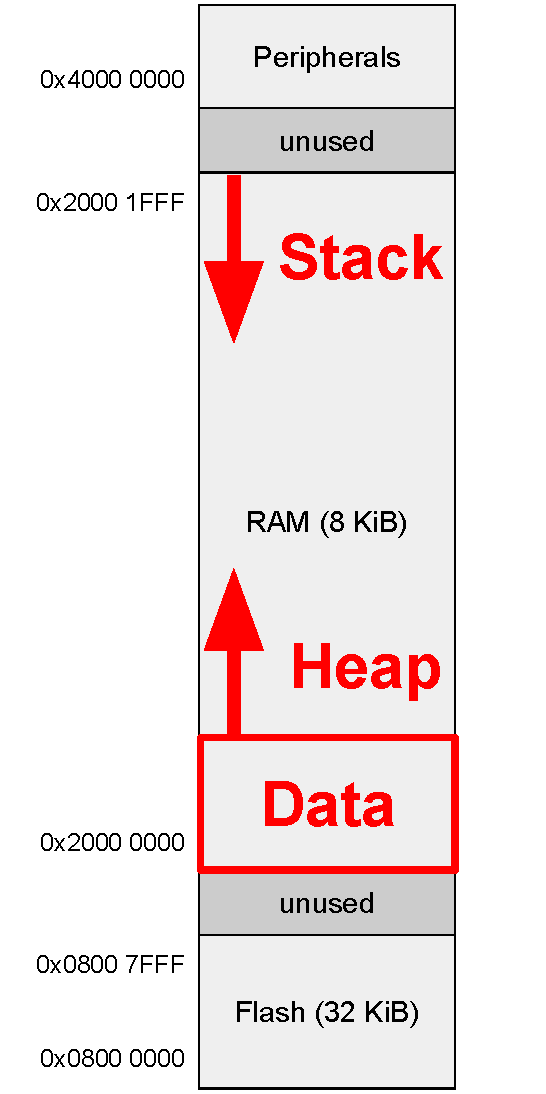
\includegraphics[scale=0.7]{./fig/mem_allocation.pdf}
    \caption{Layout of different variable blocks in memory. Note how data is fixed at compile time while stack and heap grow dynamically}
    \label{fig:mem_allocation}
\end{figure}

\subsection{Initialisation}
As stated previously:
\begin{itemize}
  \item Statically allocated variables are expected to be initialised by the time your main C code runs
  \item These variables have a fixed location at the start of RAM
  \item We know how the .bss section gets initialised: store start and end address of section and zero everything in between
\end{itemize}
How does the initialisation procedure work for the .data section? In other words, the variables which are initialised to non-zero values.
Naturally, the initialisation values have to be stored in flash such that they are not lost when power is switched off.
These initialisation values must then be copied from flash to RAM when the micro resets, in the startup code, before the C code runs.

How is this achieved? 
So far in our linker scripts we have only defined \emph{one} location for sections. That location refers both to where in memory the contents of that section are placed when we load the code from the computer onto the micro and also where in memory the symbols defined in that section will be considered to be when we use those symbols at \emph{run time}. These two types of location are called the Load Memory Address (LMA) and Virtual Memory Address (VMA) respectively.

In the majority of cases, having the VMA and LMA the same makes complete sense. Wherever we load sections into memory is where we expect those sections to be when we interact with them.
This is not the case for the .data section, the section with holds statically allocated variables with non-zero initialisation values. 
For this section, we want to load the initial values of the contents of the section into flash, but then interact with the section in RAM.
Naturally, this implies that we will need to ourselves copy the values from the LMA of .data to the VMA such that the VMA gets initialised. This is done with logic in the startup code.

We said that by default the VMA and LMA are the same. How do we make them different? There is parameter we can add to an output section definition in a linker script which will define a different LMA for that section. This is the \textbf{AT>} parameter.

\section{Code Implementation}
The following is a simple example showing where and how different storage class variables are defined.

\begin{lstlisting}[language=C]
int8_t foo;                 // global static variable. Defaults to 0.
void someFunction(void) {
    int8_t bar;            // local automatic variable. `Random' value.
    static int16_t baz;     // local static variable. Defaults to 0.
}
\end{lstlisting}


\section{Arrays}
An array is a group of 1\footnote{As per C99 you can have zero-length array or flexible length arrays.} or more elements, each being of the same data type.
The array occupies an amount of memory equal to the sum of the memory required for each element. An array should be define in one of two different ways:
\begin{enumerate}
    \item Specifying the value for each element as an initialiser. In this case you do not need to specify the size of the array as it will be calculated by the compiler by counting the number if element values supplied.
    \item By specifying the size of the array and no initial values. Here the memory is allocated but no values is set for each element. If the array is a static variable, each element will be initialised to 0 by the startup code. If the array is an automatic variable each element will just be garbage by default. 
\end{enumerate}

An example of both of these ways is demonstrated below.


\begin{lstlisting}[language=C]
// The compiler allocates 5 bytes sets each to the specified value
int8_t foo[] = {0xAA, 0x42, 0x69, 0x55, 0xF0};

// The compiler allocates 15 words and leaves values as default
uint32_t bar[15];
\end{lstlisting}

The variable name (in the above example \texttt{foo} or \texttt{bar}) of an array type behaves in much the same way as if it were the address of element 0 of the array. 
It is said that the variable name of an array type \emph{decays} to a pointer type.
This means that you cannot write to the variable name, as it makes no sense to modify the address of element 0 after it has already been defined. 
Should you wish to access the element, you should first \emph{dereference} the variable which will give you access to the data. 
Should you wish to access element 1, you should add 1 to the address of element 0 and then deference that. 
This will always work independent of the size of the elements of the array due to arithmetic operations applied to pointer types working in multiplies of the size of the data being pointed to by the pointer, as discussed earlier.

There is a nice shorthand for accessing elements of arrays; the square bracket operator. This operator just dereferences the pointer plus some number. The following two are equivalent. 
\begin{lstlisting}[language=C]
*(myArray + 10);
myArray[10];
\end{lstlisting}

Note that although the square bracket operator is most useful on array types, it is valid on any pointer types. 

\section{Structs}
An array is limited in that each element of the array must be of the same type. A struct seeks to overcome this by allowing you to create a custom data structure which has elements (now called `members') of different data types. Additionally, rather than accessing the members via an index as you would do for an array, you access the members via their names. 
Our main use for structs will be in interfacing with peripherals.
A peripheral can be modeled as a struct where each register has a name and is of a potentially different size to the other registers in the peripheral.

There are two defining a variable of struct type.
The first step is to declare the struct. The second step is to define a variable of that type.
The struct declaration specified what the struct looks like in terms of struct name, member sizes and member names.

\begin{lstlisting}[language=C]
struct myStruct {
    uint32_t  member1;
    uint8_t   *member2;
    uint8_t   member3[8];
    int32_t   member4; 
};
\end{lstlisting}

Once that code is in place, you can then define variables of type \texttt{struct myStruct}. This may seem hairy, but it is a variable just like any other and defined in the same way.

\begin{lstlisting}[language=C]
struct myStruct foo;
\end{lstlisting}

The variable \texttt{foo} is now of a variable of type \texttt{struct myStruct}. What can you do with this variable? Well, just like how you can access the elements of an array, you can access the members of a struct. This is done via the member access operator, the full stop / dot. 

\begin{lstlisting}[language=C]
foo.member1 = 0xAABBCCDD;
foo.member2 = &someVar;
foo.member3[6] = 0xAA;    // member 3 is an array
foo.member3[7] = 0xBB;
foo.member4 = -42;
\end{lstlisting}

\subsection{Memory Layout}
How does this struct appear in memory? This is key to understand as we want our struct to map exactly to the memory layout of the registers of a peripheral. 
Firstly, note that when we declared the variable \texttt{foo}, we had no control where the memory for this struct was allocated. This is troublesome, but let's ignore that for now.

The struct requires a certain amount of space to be allocated to it. How much space? The sum of the space for each member. 
\begin{align*}
size &= \texttt{ member1 } + \texttt{ member2 } + \texttt{ member3 } + \texttt{ member4 }\\
 &= 4 + 4 + (8*1) + 4\\
 &= 20 \text{ bytes}
\end{align*}

That is to say, whenever a variable of type \texttt{struct myStruct} is defined, 20 bytes must be allocated for it. 

Typically, the members are laid out in the order which they are specified in. Things start to become more complicated when you have alignment issues or memory optimisation requirement, but we will ignore those for our alanysis of structs. 

Wherever the variable \texttt{foo} happens to get allocated in memory, \texttt{member1} will have an offset of 0 and occupy 4 bytes while \texttt{member2} will have an offset of 4 and occupy 4 bytes while \texttt{member3} will have an offset of 8 and occupy 8 bytes while \texttt{member4} will have an offset of 16 and occupy 4 bytes. 

\subsection{Pointers To Structs}
As mentioned, the most useful application of structs for us is interfacing with out peripherals. For that we need to have precise control over where the struct is placed in memory. Unfortunately, this is not possible as the compiler always decides where memory is allocated. 
However, do have a tool which allows us to `fake' structs anywhere in memory. This is the exact same tool which we used when we first stated interfacing with registers.
Recall that we interfaced with peripheral registers as follows.

\begin{lstlisting}[language=C]
// treat the number as a pointer to a uint32_t and dereference it.
*(uint32_t *)0x48000040 = 0x5555;
\end{lstlisting}

That is saying "treat 0x4800 0040 as a pointer to a 32-bit number, access the data being pointed to and write 0x5555 to it." We can do the exact same thing for structs!
\begin{lstlisting}[language=C]
// treat the number as a pointer to a myStruct, dereference it,
// and access a member.
(*(struct myStruct *)0x48000040).member1 = 0x5555;  
\end{lstlisting}

That will write the number 0x5555 to the base address 0x4800 0040 plus the offset of \texttt{member1} which is an offset of 0.
Similarly, we could do something like the following which would write to the 8-bit number located at base address 0x4800 0040 plus offset of $4 + 4 + (4*1) = 12 = \text{0x0C}$. 
\begin{lstlisting}[language=C]
(*(struct myStruct *)0x48000040).member3[4] = 0xAA;  
\end{lstlisting}

Notice what we are doing in the previous two examples: we are dereferencing a pointer to a struct and then accessing a member of that struct.
This operation of dereferencing and then accessing a member is so often done that there is an operator for it, the \emph{indirect} member access operator: \texttt{->}.
Using this operator, the above two examples can be re-written more elegantly as follows.
\begin{lstlisting}[language=C]
((struct myStruct *)0x48000040)->member1 = 0x5555;  
((struct myStruct *)0x48000040)->member3[4] = 0xAA;  
\end{lstlisting}

Just like we can define variables of struct type, we can also define variables of pointer to struct type.
The above example could also be implemented with a variable declaration as follows. 

\begin{lstlisting}[language=C, frame=trBL]
// do explicit typecast to prevent compiler warning
struct myStruct *foo = (struct myStruct*)0x48000040;
foo->member1 = 0x5555;
foo->member3[4] = 0xAA;
\end{lstlisting}

This implementation using a variable is \emph{less} efficient as it requires a pointer variable to be allocated in memory and accessed. With the previous implementations which did not use a variable all of the addresses are resolved at compile time which makes the program faster and smaller. 
